\section{Theorie}
\subsection{Theorie des Lichts}
Ein Laser emittiert hoch intensives monochromatisches Licht, also Licht einer einzigen Wellenlänge beziehungsweise Farbe. Das bedeutet auch, dass das Licht möglichst kohärent ist, also der Kontrast der Interferenzmuster maximiert wird. In der Realität ist das Licht nicht perfekt monochromatisch, da im Lasergehäuse die Neonatome nicht still stehen, sondern eine eigene Geschwindigkeit haben und somit der Doppler-Effekt bezüglich des emittierten Lichts eintritt. Somit ist auch die perfekte Kohärenz nicht möglich.

\noindent Licht wird im Teilchenbild durch Emission von Photonen beim Übergang eines Elektrons von einem Niveau eines Atoms in ein energetisch günstigeres beschrieben. Es existieren zwei Arten der Emission. Die stimulierte und spontane Emission. Die spontane Emission entsteht durch Fluktuationen in der Ladungsverteilung der Atome. Die stimulierte Emission ist die für den Laser relevante, da dabei im Gegensatz zum statistischen Ereignis der spontanen Emission, die Abstrahlung von Photonen kontrolliert werden kann. Dabei werden zwei Photonen emittiert, von denen eines die selbe Energie, Phase und Ausbreitungsrichtung wie das stimulierende beziehungsweise einfallende Photon hat.

\noindent Darüber hinaus gibt es noch die Absorption. Hierbei wird ein auf das Atom treffende Photon, welches die Energie des Überganges hat, absorbiert indem ein Elektron ein Energieniveau aufsteigt.

\noindent Ein zwar nicht für die Funktion eines Lasers ausreichendes, aber grundlegendes System ist das Zwei-Niveau-System. Dabei wird die Besetzungsdichte \(n_2\) des angeregten Zustandes durch die Absorption erhöht und durch die spontane und stimulierte Emission verringert. Um hochintensive Licht zu erzeugen, sollte bei einem Laser die stimulierte Emission der Absorbtion überwiegen, sodass das \(n_2>n_1\) ist, wobei \(n_1\) die Besetzungsdichte im Grundzustand bedeutet.

\subsection{Theorie des Lasers}
Ein Laser besteht im wesentlichen aus drei Komponenten. Eine ist das aktive Lasermedium. Dabei handelt es sich um ein Gas, einen Festkörper oder eine Flüssigkeit. Bei dem Laser dieses Versuchs wird ein Gas verwendet. Die notwendige Bedingung an ein Lasermedium stellt die Fähigkeit zur Besetzungsinversion dar, also \(n_2>n_1\). Als Lasermedium dient hier Neon.

\noindent Eine weitere Komponente ist die Pumpquelle. Durch das so genannte Pumpen, wird dem Lasermedium Energie zugeführt und somit Zustände höherer Energie häufiger besetzt, als diejenigen niedrieger. Es wird also eine Besetzungsinversion erzeugt. Entscheidend dafür, ob ein Niveau durch pumpen angeregt werden kann, ist die Temperatur des Systems, also die Besetzung der Niveaus bezüglich der Boltzmann-Verteilung, die Anregungsrate sowie die Lebensdauer der Zustände im angeregten Zustand. Die Energie wird an das Neon durch Stöße zweiter Art übergeben. Diese sind Stöße zweier Atome, von denen eines im Angeregten und das andere im Grundzustand ist. Bei einem Stoß zweiter Art besteht dann eine Wahrscheinlichkeit, das angeregte Atom in den Grundzustand und das im Grundzustand verweilende in den angeregten Zustand zu bringen. Die Pumpquelle ist hier Helium. Das Verhältnis von Helium zu Neon ist bei diesem Laser fünf zu eins.

\noident Die dritte Komponente ist der Resonator. Er besteht aus einem möglichst vollständig reflektierenden und einem teildurchlässigen Spiegel sowie einem Laserrohr, in dem sich das Lasermedium befindet und das an den Enden in Brewsterfenster mündet. Die Brewsterfenster sind 

%BREWSTERFENSTER ERKLÄREN

. Diese stehen in einem Abstand \(L\)  voneinander auf der optischen Achse und haben die Krümmungsradien \(r_1\) und \(r_2\). Dadurch entsteht eine optische Rückkopplung, bei der das Licht mehrmals das Lasermedium durchläuft und ein selbsterregender Oszillator entsteht. 

\noindent Ein grober Aufbau eines Resonators ist in Abbildung \ref{fig:hene1} gegeben.

\begin{figure}
	\centering
		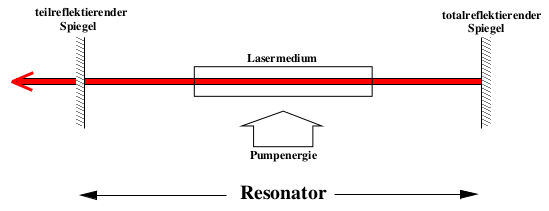
\includegraphics[width=0.5\textwidth]{hene1.png}
	\caption{Laser-Resonator}
	\label{fig:hene1}
\end{figure}

\noindent Durch den Resonator legt der Laserstrahl einen möglichst langen Weg im Lasermedium zurück und wird somit verstärkt. Die Stabilität ist daher vom Resonatortyp und der Form der Spiegel abhängig. Optimal sind für einen Laser konfokale Spiegel, da diese einen in einem Punkt zusammenfallenden Brennpunkt gewährleisten und somit geringe Verluste bezüglich der Resonatorspiegel aufweisen.

\noindent Eine Stabilitätsbedingung für den Resonator ist gegeben durch:

\begin{equation}
\label{eq:1}
0\le g_1\cdot g_2<1
\end{equation}

\noindent Dabei sind die \(g_i\) durch \(g_i=1-\frac{L}{r_i}\ gegeben.

\noindent Es existiert eine Mehrzahl von Frequenzen, die die Resonanzbedingung erfüllen. Diese sind über \(f=\frac{nc}{\pi L}\) gegeben. Es gibt sowohl transversale als auch longitudinale Moden. Erste entstehen, durch Unebenheiten der Spiegel oder Verkippungen. Die Moden werden als \(\text{TEM}_{lpq}\) (transverse electromagnetic mode) bezeichnet, dabei sind \(l\) und \(p\) die Knoten in x- und y-Richtung und heißen transversale Modenzahl. Die Verluste steigen mit der Modenzahl, sodass nur wenige Moden isoliert werden können. Die Mode mit höchster Symmetrie und mit den wenigsten Verlusten ist die \(\text{TEM}_00\) Grundmode.